\section{Künstliche Neuronale Netze}
\label{chap:networks}
\info{Die Theorie zu neuronalen Netzen ist fast vollständig, nur über ConvNets würde ich noch mehr schreiben wollen.}
Künstliche neuronale Netze (KNN), häufig auch nur neuronale Netze genannte, haben in den letzten Jahren das Forschungsfeld des maschinellen Lernens revolutioniert. Die Ideen hinter KNNs stammen aber bereits aus den 1940ern und 1950ern.McCulloch und Pitts haben 1943 ein Modell der Neuronen als Recheneinheit vorgestellt, das die Funktionsweise von biologischen Neuronen imitieren sollte. Basierend auf dieser Arbeit hat Frank Rosenblatt 1957 das Perzeptron (von engl. \textit{to percept}, etwas wahrnehmen) erfunden. Eine Maschine, die binäre Inputs verarbeitet und einen binären Output erzeugt. Die Besonderheit des Perzeptrons war, dass es lernen konnte, seine Parameter anzupassen wenn der erzeugte Output falsch war - es konnte lernen. Das Perzeptron ist auch heute noch die Basis für die Einheiten, aus denen neuronale Netze bestehen.
\par 
Ein Perzeptron alleine kann einfache aussagenlogische Verknüpfungen wie AND, OR und NAND implementieren, scheitert aber an XOR und anderen sogenannten nicht linear separierbaren Problemen\footnote{Zwei Mengen von Punkten $A$ und $B$ im 2-dimensionalen Raum sind linear separierbar, wenn eine Gerade so platziert werden kann, dass alle Punkte von $A$ auf einer Seite der Linie liegen und alle Punkte von $B$ auf der anderen.}, dies haben Minsky und Papert in ihrem Buch Perceptrons 1969 gezeigt.

Dieses Problem wurde so schlimm von der Forschungsgemeinde aufgenommen, dass das Interesse an Perzeptrons verebbte.

Abhilfe schaffte der sogenannte Multi layer Perceptron (MLP), ein mehrschichtiges Netzwerk aus Perzeptronen, allgemeiner einfach nur Neuronen bezeichnet. Durch die Verknüpfung mehrerer Neuronen konnten auch komplexere Probleme wie das XOR Problem gelöst werden, doch das Training eines solchen Netzwerks hat lange für Schwierigkeiten gesorgt. Erst in den 80ern wurde es durch Anwendung des sogenannten Backpropagation Algorithmus mit Hilfe von automatischer Differenzierung möglich auch tiefere neuronale Netze zu trainieren.\\

Die Erfolge beim Kombinieren von Monte-Carlo Baumsuche mit neuronalen Netzen um Brettspiele wie Go, Shogi und Schach zu lernen von Silver et. al\cite{silverMastering}, macht mich zuversichtlich, dass neuronale Netze auch Vier Gewinnt gut lernen können.

\subsection{Neuronen}

\begin{figure}[!hbt]
	\centering
	\begin{tikzpicture}
	[x=1.5cm,y=1.5cm,>=stealth,
	neuron/.style={circle,draw,inner sep=2pt, minimum size=1cm},
	aktiv/.style={rectangle,draw,inner sep=2pt, minimum size=1cm}]
	\node at (-1,1)  (input1) {$x_1$};
	\node at (-1,-1) (input2) {$x_2$};
	\node at (2,0) [neuron] (neuron) {$\sum$};
	\node [aktiv] (activation) [right=of neuron] {$\sigma$};
	\node (bias) [below=of neuron] {b};
	\node (output) [right=of activation] {Output};
	\draw [->] (input1) -- (neuron) node [above, midway] {$w_1$};
	\draw [->] (input2) -- (neuron) node [above, midway] {$w_2$};
	\draw [->] (neuron) -- (activation);
	\draw [->] (bias) -- (neuron);
	\draw [->] (activation) -- (output);
	\end{tikzpicture}
	\caption{Neuron mit zwei Inputs und Bias}
\end{figure}

Neuronen sind kleine Einheiten die Inputs (\textbf{Features}) entgegennehmen und einen Output erzeugen. Sie unterscheiden sich vom Perzeptron dadurch, dass die Inputs und Outputs reelle Zahlen, in der Regel zwischen 0 und 1, sind. Jedes Neuron hat eine Menge von \textbf{Gewichten} $w$ und einen \textbf{Bias-Wert} $b$. Die Gewichte werden verwendet um eine Gewichtete Summe der Eingangssignale zu berechnen. Der Bias-Wert dient dazu zu steuern, wie leicht oder schwer das Neuron "aktiviert" wird, also wie leicht es ist einen positiven Output zu erzeugen. Man nennt die Gewichte zusammen mit dem Bias auch die \textbf{Parameter} eines Neurons. Ein Neuron mit 3 Inputs hat also 3 Gewichte und 1 Bias also 4 Parameter.


Der berechnete Wert des Neurons $z = x \bigcdot w + b$ wird dann durch eine \textbf{Aktivierungsfunktion} geschickt, um den Output des Neurons zu bestimmen. Im klassischen Perzeptron ist diese Aktivierungsfunktion die Stufenfunktion
\begin{equation}
	STEP(z) = \begin{cases}
	0 & z \le 0\\
	1 & z > 0
	\end{cases}.
\end{equation}
Die Stufenfunktion macht es aber schwer, die Parameter des Neurons präzise zu trainieren. Idealerweise führt eine kleine Anpassung der Gewichte zu einer kleinen Änderung des Outputs, die Stufenfunktion sorgt aber dafür dass die Änderung entweder nichts bewirkt oder eine große Änderung ($\pm 1$) auslöst.

Deswegen werden heute viele verschiedene Aktivierungsfunktionen eingesetzt. Die erste viel genutzte ist die Sigmoid Funktion
\begin{equation}
\sigma(z) = \frac{1}{1 + e^{-z}}
\end{equation}
Sie wird, genauso wie die Stufenfunktion, für große positive Werte 1 und für große negative Werte 0, dazwischen steigt sie aber stetig an. Sie hat somit das gewünschte Verhalten, dass kleine Veränderungen im Input nur einen kleinen Einfluss auf den Output haben.

Ein Neuron ohne Aktivierungsfunktion würde auch funktionieren, verliert dann aber kombiniert in einem Netzwerk seine Wirkung. Jedes Neuron für sich berechnet eine Linearkombination seiner Inputs. Eine Kombination dieser Neuronen führt dazu, dass der Output ebenfalls nur eine Linearkombination der Inputs des Netzwerks ist. Egal wieviele Schichten das Netzwerk hat, der Output verhält sich so als gäbe es nur eine Schicht. Aktivierungsfunktionen sind daher nicht-linear, wodurch sich jede beliebige Funktion approximieren lässt.\\

Es gibt noch viele weitere Aktivierungsfunktionen die für neuronale Netze benutzt werden. Nachfolgend ein paar Beispiele:
\label{chap:activations}
\paragraph{tanh} Die Sigmoid Funktion ist eigentlich ein gestauchter und verschobener Tangens hyperbolicus $tanh(z) = \frac{e^z-e^{-z}}{e^z+e^{-z}}$. $tanh(z)$ hat daher eine ähnliche Form wie die Sigmoid Funktion, ihr Wertebereich ist aber $(-1,1)$
\paragraph{ReLU} ReLU steht für \textbf{Re}ctified \textbf{L}inear \textbf{U}nit und ist eine sehr einfache Funktion: $RELU(z) = max(0, z)$. Der Wert von ReLU ist 0 für alle $z < 0$ und sonst $z$. Diese Aktivierungsfunktion leidet an dem Problem, dass negative Werte und Werte nahe 0 dafür sorgen, dass das Neuron keine Aktivierung mehr hat, das Neuron "stirbt".
\paragraph{Leaky ReLU} Leaky ReLU versucht das Sterben des Neurons zu verhindern, indem auch der negative Teil eine kleine Steigung hat. $LEAKY(z) = max(\alpha z,z)$ mit einem kleinen $\alpha$.\\\\

Die Aktivierungsfunktionen müssen differenzierbar sein, da die Ableitung für das Training im Backpropagation Algorithmus verwendet wird.

\subsection{Architektur eines Neuronalen Netzes}

\def\layersep{2.5cm}
\def\nodesize{1cm}
\begin{figure}[!hbt]
	\centering
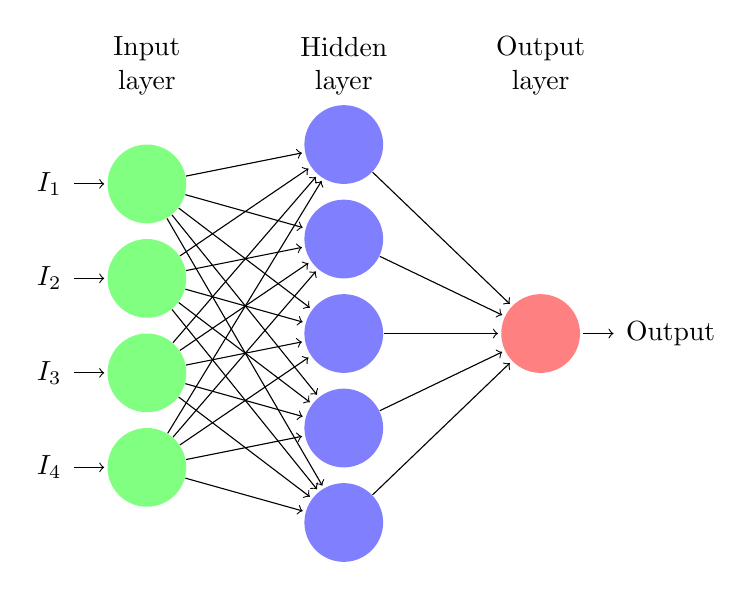
\begin{tikzpicture}[shorten >=1pt,->,draw, node distance=\layersep]
\tikzstyle{every pin edge}=[<-,shorten <=1pt]
\tikzstyle{neuron}=[circle,fill=black!25,minimum size=\nodesize,inner sep=0pt]
\tikzstyle{input neuron}=[neuron, fill=green!50];
\tikzstyle{output neuron}=[neuron, fill=red!50];
\tikzstyle{hidden neuron}=[neuron, fill=blue!50];
\tikzstyle{annot} = [text width=4em, text centered]

% Draw the input layer nodes
\foreach \name / \y in {1,...,4}
% This is the same as writing \foreach \name / \y in {1/1,2/2,3/3,4/4}
\node[input neuron, pin=left:$I_\y$] (I-\name) at (0,-\y*1.2*\nodesize) {};

% Draw the hidden layer nodes
\foreach \name / \y in {1,...,5}
\path[yshift=0.5cm]
node[hidden neuron] (H-\name) at (\layersep,-\y*1.2*\nodesize) {};

% Draw the output layer node
\node[output neuron,pin={[pin edge={->}]right:Output}, right of=H-3] (O) {};

% Connect every node in the input layer with every node in the
% hidden layer.
\foreach \source in {1,...,4}
\foreach \dest in {1,...,5}
\path (I-\source) edge (H-\dest);

% Connect every node in the hidden layer with the output layer
\foreach \source in {1,...,5}
\path (H-\source) edge (O);

% Annotate the layers
\node[annot,above of=H-1, node distance=1cm] (hl) {Hidden layer};
\node[annot,left of=hl] {Input layer};
\node[annot,right of=hl] {Output layer};
\end{tikzpicture}
\caption{Ein neuronales Netz mit 2 Schichten, die Eingabeschicht wird nicht mitgezählt}
\label{fig:neuralnetwork}
\end{figure}

Neuronale Netze bestehen aus mehreren Schichten mit jeweils einem oder mehreren Neuronen. Die erste Schicht ist der \textbf{Input layer} (Eingabeschicht). Häufig werden die Inputs als Neuronen dargestellt, mit einem Neuron pro Input-Feature. Die Neuronen der Eingabeschicht reichen nur ihren jeweiligen Input an die nächste Schicht weiter. Generell wenn die Rede ist von einem neuronalen Netz mit $n$ Schichten, so wird die Eingabeschicht nicht mitgezählt (siehe Abb. \ref{fig:neuralnetwork}).
\par 
Alle Schichten zwischen der ersten und letzten Schicht werden als \textbf{Hidden layer} (versteckte Schichten) bezeichnet. In einem einfachen neuronalen Netz sind alle Neuronen mit allen Neuronen der vorherigen Schicht verbunden, man spricht von vollständig verbundenen Schichten (fully connected layers oder auch "dense" layers). Die Neuronen in den versteckten Schichten haben häufig eine andere Aktivierungsfunktion als der Output. Generell könnte jedes Neuron eine eigene Aktivierungsfunktion besitzen, in der Praxis ist es aber üblich, dass alle Neuronen einer Schicht die selbe Aktivierungsfunktion haben. Während anfangs die Sigmoid Funktion für die versteckten Schichten bevorzugt wurde, da diese Aktivierung der der biologischen Neuronen am nächsten kommt, wird heutzutage häufig ReLU eingesetzt.
\par 
Die letzte Schicht wird \textbf{Output layer} (Ausgabeschicht) genannt. Die Ausgabeschicht besteht aus einem Neuron für jeden Zielwert. Ein Netzwerk für die Bestimmung eines Hauspreises zum Beispiel hat nur ein Output Neuron, ein Netzwerk für die Klassifizierung von handgeschriebenen Ziffern dagegen hat ein Neuron für jede mögliche Ziffer 0 bis 9. Die Aktivierungsfunktion der Ausgabeschicht ist davon abhängig, welche Aufgabe das neuronale Netz lösen soll.\\
\par 
Die Gewichte der Verbindungen zwischen Neuronen werden in der Regel als eine Matrix repräsentiert, während die Inputs einer Schicht und die Bias-Werte Vektoren sind. Somit lässt sich durch lineare Algebra einfach die Aktivierung einer Schicht $L$ mit Aktivierungsfunktion $\sigma$ berechnen durch
\begin{equation}
	a^L = \sigma(w^L\cdot a^{L-1} + b^L).
\end{equation}
Ist $L$ die erste versteckte Schicht, so ist $a^{L-1}$ der Vektor der Inputs. Jede Zeile der Matrix entspricht dabei den Gewichten eines Neurons und jede Spalte den Inputs in die Schicht.\\

\par
Neuronale Netze werden für die verschiedensten Aufgaben verwendet, die Hauptanwendungsfälle lassen aber in Klassifizierung und Regression aufteilen.
\label{chap:regression-classification}
\paragraph{Klassifizierung} Das Ziel der Klassifizierung ist es, die Beispiele, die das System verarbeitet, in Klassen einzuteilen - es sollen diskrete Werte vorhergesagt werden. Unterschieden wird hierbei zwischen \textbf{binärer Klassifizierung}, \textbf{multi-label Klassifizierung} und \textbf{multi-class Klassifizierung}.\\
Die \textit{binäre Klassifizierung} stellt die Frage, ob das Beispiel zur Klasse gehört oder nicht, der gewünschte Output also 1 ist. \\
Die \textit{multi-label Klassifizierung} ist eine Art parallele binäre Klassifizierung. Es gibt mehrere Zielklassen und das Beispiel kann zu einer oder mehreren dieser Klassen gehören, entsprechend gibt es in diesem Fall so viele Outputs wie es Klassen gibt und die Outputs der Zielklassen müssen 1 werden.\\
Die \textit{multi-class Klassifizierung} hat ebenfalls mehrere Zielklassen, allerdings gehört das Beispiel nur zu einer der Klassen.\\
\par 
Eine typische Aktivierungsfunktion für die Klassifizierung ist die Sigmoid Funktion. Für die multi-class Klassifizierung wird in der Regel die Softmax Funktion eingesetzt. Ihr Ergebnis ist eine Wahrscheinlichkeitsverteilung über alle Zielklassen die sich zu eins aufsummiert.

\paragraph{Regression} Regressionsaufgaben sind Aufgaben, bei denen ein kontinuierlicher Zielwert vorhergesagt werden soll. Zum Beispiel der Preis eines Hauses basierend auf Informationen wie der Lage, dem Baujahr und der Fläche des Grundstücks. Für die Regression hat das neuronale Netz einen Output für jeden Zielwert, der vorhergesagt werden soll.\\
\par 
Für Regression wird häufig keine Aktivierungsfunktion benutzt, wenn ein skalarer Wert wie ein Preis bestimmt werden soll. Liegt der Zielwert dagegen in einem bestimmten Wertebereich, so kann auch hier die Sigmoid oder tanh Funktion verwendet werden. Soll der Wert immer positiv sein, so kann die ReLU Funktion eingesetzt werden.\\


\par 
Ein neuronales Netz mit nur einer versteckten Schicht wird in der Literatur häufig als flaches Netzwerk und eines mit mehreren Schichten als tiefes Netzwerk (deep network) bezeichnet. Heutzutage sind Netzwerke mit 3 bis 10 Schichten nicht selten, weshalb der Begriff eines "tiefen Netzwerks" etwas schwammig geworden ist.

\subsection{Training eines Neuronalen Netzes}

Bevor ein neuronales Netz eingesetzt werden kann, muss es zunächst angelernt werden. Für dieses Training ist eine große Menge an Trainingsdaten notwendig und das neuronale Netz muss diese Trainingsdaten mehrfach durchlaufen, bis es sichere Vorhersagen treffen kann. Jeder Durchlauf durch die gesamten Trainingsdaten wird als \textbf{Epoche} (engl. epoch) bezeichnet. Jedes Beispiel der Trainingsdaten besteht aus Features, den Eingabewerten in das neuronale Netzwerk, und Zielwerten. Das Netzwerk lernt dabei die Zusammenhänge zwischen den Features und den Zielwerten.
\\

\subsubsection{Fehlerfunktion}
\label{chap:cost-function}

In jedem Durchlauf durch diese Trainingsdaten wird mit einer \textbf{Fehlerfunktion} der Fehler des Netzwerks berechnet. Also wie sehr das Netzwerk im Durchschnitt mit seinen Vorhersagen daneben lag. Die Fehlerfunktion (engl. cost function) muss abhängig von der Aufgabe und der Art der Trainingsdaten gewählt werden. 
\par 
Für Regression wird häufig der durchschnittliche Fehler im Quadrat (engl. mean squared error, MSE) oder, wenn es viele Ausreißer in den Daten gibt, der mittlere absolute Fehler (engl. mean absolute error, MAE) berechnet.\\

Im folgenden gilt: $y$ ist der Zielwert, $\hat{y}$ ist die Vorhersage des Netzwerks, $m$ ist die Anzahl der Trainingsbeispiele und die Indexierung $y_i$ bezeichnet das $i$-te Beispiel im Trainingsdatensatz.

\begin{equation}
\label{eqn:mse}
	MSE = \frac{1}{m}\sum_{i=1}^{m}(y_i-\hat{y}_i)^2
\end{equation}
\begin{equation}
\label{eqn:mae}
	MAE = \frac{1}{m}\sum_{i=1}^{m}|y_i-\hat{y}_i|
\end{equation}

Eine typische Fehlerfunktion für Klassifizierung ist die (binäre) Kreuzentropie (engl. cross entropy loss). Damit werden Wahrscheinlichkeitsverteilungen miteinander verglichen.

\begin{equation}
\label{eqn:crossentropy}
CrossEntropy = -\frac{1}{m}\sum_{i=1}^{m} [y_i\ln(\hat{y}_i)+(1-y_i)\ln(1-\hat{y}_i)]
\end{equation}

Der Fehler ist gering, wenn die Vorhersage sehr nahe an dem erwarteten Wert ist, und wird groß wenn die Vorhersage stark abweicht. Wichtig ist, dass diese Fehlerfunktionen den Fehler über den gesamten Trainingsdatensatz berechnen.\\
\par 
Die Vorhersagen des Netzwerks, und damit auch der Fehler, hängen direkt von den Parametern (Gewichten) des Netzwerks ab. Da die Trainingsbeispiele statisch sind, kann der Fehler nur reduziert werden, indem die Parameter des Netzwerks verändert werden. Effektiv ist die Fehlerfunktion also eine Funktion der Parameter des Netzwerks. Das Ziel ist es, diese Parameter so anzupassen, dass die Fehlerfunktion minimiert wird. Das verwendete Optimierungsverfahren ist auch als Gradientenverfahren (engl. gradient descent) bekannt.

\subsubsection{Gradientenverfahren und Backpropagation}

Stell dir vor du stehst auf einem Berg umrandet von Bäumen und willst das Tal erreichen, du siehst aber nicht wo genau es sich befindet. Der Boden unter deinen Füßen ist leicht geneigt. Solange du dich immer in Richtung der größten Steigung bewegst, wirst du irgendwann ein Tal erreichen. Nach diesem Prinzip funktioniert auch das Gradientenverfahren.\\
\par 
Der Berg, dessen Tal wir erreichen wollen, ist die Fehlerfunktion und die Steigung dieser Funktion wird durch die Gewichte des neuronalen Netzes bestimmt. Wenn wir für jedes Gewicht, also jede mögliche "Richtung" in einem $n$-dimensionalen Raum, die Steigung an der aktuellen Position (mit den aktuellen Parametern) berechnen, so können wir alle Gewichte ein kleines bisschen verändern und uns dem Tal Schritt für Schritt nähern.
\par 
Die Steigung ist, wie aus der Analysis bekannt, die Ableitung der Funktion in Abhängigkeit vom Parameter $C'(x) = \frac{\delta C}{\delta x}$. Für jeden Parameter des Netzwerks muss diese partielle Ableitung berechnet werden. Ein Vektor mit allen diesen partiellen Ableitungen wird auch als Gradient bezeichnet $\nabla C(w_{1,1},w_{2,1},...,w_{k,n}) = (\frac{\delta C}{\delta w_{1,1}}, \frac{\delta C}{\delta w_{2,1}}, ..., \frac{\delta C}{\delta w_{k,n}})^T$, daher der Name Gradientenverfahren.\\
\par 
Die Berechnung der Ableitungen geschieht im Backpropagation Algorithmus. Nachdem die Trainingsbeispiele durch das Netzwerk geführt wurden und der Fehler bestimmt wurde, wird jetzt der Fehler rückwärts durch das Netzwerk zurückgeführt. Zunächst wird für jeden Output bestimmt, welchen Einfluss er auf den Fehler hatte. Durch Anwendung der Kettenregel wird dann die Beteiligung jeder Verbindung - die Ableitung des Fehlerfunktion in Abhängigkeit vom Gewicht der Verbindung - der vorherigen Schicht berechnet. Der Algorithmus arbeitet sich Schicht für Schicht durch das Netzwerk, bis die Eingabeschicht erreicht ist. Nachdem auf diese Weise alle partiellen Ableitungen bestimmt sind, kann nun ein Schritt des Gradientenverfahrens durchgeführt und die Parameter etwas verbessert werden.\\
\par 
Es gibt viele Optimierungen des Gradientenverfahrens \autocite[\ppno~50]{cholletDeepLearningPython2017}. Eine der gängigsten Erweiterungen fügt ein Momentum hinzu, was konzeptionell ähnlich ist wie wenn nicht ein Mensch einen Berg hinabsteigt, \change{Formulierung}sondern ein Ball hinab rollt. Der Ball bewegt sich noch ein bisschen in die Richtung des letzten Updates weiter, er verhält sich also träge. Dadurch kann der Algorithmus aus lokalen Minima hinausrollen und schafft es so mit größerer Wahrscheinlichkeit in ein globales Minimum. Andere Verfahren verändern die Lernrate des Algorithmus für individuelle Parameter.

\subsection{Convolutional Neural Networks}

Convolutional neural Networks (ConvNets) orientieren sich am menschlichen Sehen und der Funktionsweise des visuellen Kortex. In einem großen Bild, das das Auge sieht, hat jedes Neuron des visuellen Kortex nur ein kleines rezeptives Feld. Es ist nur Empfindlich auf Muster, die in diesem Feld auftauchen. Dieses Konzept wird durch Kernelfilter auf neuronale Netze übertragen. Kernelfilter finden unter anderem in der Bildbearbeitung und Signalverarbeitung Anwendung. So wird zum Beispiel die Schärfe und Unschärfe-Funktion eines Bildbearbeitungsprogramms durch einen Kernelfilter umgesetzt. 

\improvement[inline]{Hier sollte eine Grafik der Kernel-Anwendung hin}

Ein Kernelfilter ist eine kleine quadratische Matrix, meistens 3x3 oder 5x5, die Pixel für Pixel über ein Bild geschoben wird. Für jeden Pixel werden alle umliegenden Pixel mit den Werten des Filters multipliziert und dann der Durchschnitt gebildet, um den neuen Wert für den mittleren Pixel zu bestimmen. 

Klassische neuronale Netze mit einem Neuron für jedes Input Feature können auch auf Bilder angewandt werden indem für jedes Pixel und jeden Farbkanal ein Input-Neuron verwendet wird. Dadurch steigt allerdings die Größe des Netzwerks explosionsartig, gerade wenn Bilder mit Millionen von Pixeln verarbeitet werden. Ein solches neuronales Netz erkennt globale Muster in den Eingabedaten, so sind zum Beispiel die ersten 5 Neuronen der ersten verstecken Schicht aktiv, wenn ein bestimmtes Muster in der oberen linken Ecke auftaucht. Kernelfilter und Kernelfilter-Schichten suchen dagegen nach lokalen Mustern. Da der Filter über das gesamte Bild bewegt wird, ist er an allen Stellen aktiv, an denen das lokale Muster im Fenster auftaucht. Kernelfilter werden auch als Translationsinvariant bezeichnet.